\documentclass[a4paper, 14pt]{extarticle}

% Поля
%--------------------------------------
\usepackage{geometry}
\geometry{a4paper,tmargin=2cm,bmargin=2cm,lmargin=3cm,rmargin=1cm}
%--------------------------------------


%Russian-specific packages
%--------------------------------------
\usepackage[T2A]{fontenc}
\usepackage[utf8]{inputenc} 
\usepackage[english, main=russian]{babel}
%--------------------------------------

\usepackage{textcomp}

% Красная строка
%--------------------------------------
\usepackage{indentfirst}               
%--------------------------------------             


%Graphics
%--------------------------------------
\usepackage{graphicx}
\graphicspath{ {./images/} }
\usepackage{wrapfig}
%--------------------------------------

% Полуторный интервал
%--------------------------------------
\linespread{1.3}                    
%--------------------------------------

%Выравнивание и переносы
%--------------------------------------
% Избавляемся от переполнений
\sloppy
% Запрещаем разрыв страницы после первой строки абзаца
\clubpenalty=10000
% Запрещаем разрыв страницы после последней строки абзаца
\widowpenalty=10000
%--------------------------------------

%Списки
\usepackage{enumitem}

%Подписи
\usepackage{caption} 

%Гиперссылки
\usepackage{hyperref}

\hypersetup {
 unicode=true
}

%Рисунки
%--------------------------------------
\DeclareCaptionLabelSeparator*{emdash}{~--- }
\captionsetup[figure]{labelsep=emdash,font=onehalfspacing,position=bottom}
%--------------------------------------

\usepackage{tempora}


\documentclass{article}
\usepackage[utf8]{inputenc}
\usepackage[russian]{babel}
\usepackage{listings}
\usepackage{xcolor}

\lstset{
    basicstyle=\ttfamily, 
    breaklines=true,
    columns=fullflexible,
    frame=single,
    inputencoding=utf8,
    extendedchars=true,
    keywordstyle=\bf,       % keyword style
    numbers=left,                    % where to put the line-numbers; possible values are (none, left, right)
    numbersep=5pt,                   % how far the line-numbers are from the code
    xleftmargin=25pt,
    xrightmargin=25pt,
} 


%--------------------------------------
%   НАЧАЛО ДОКУМЕНТА
%--------------------------------------

\begin{document}

%--------------------------------------
%   ТИТУЛЬНЫЙ ЛИСТ
%--------------------------------------
\begin{titlepage}
\thispagestyle{empty}
\newpage


%Шапка титульного листа
%--------------------------------------
\vspace*{-60pt}
\hspace{-65pt}
\begin{minipage}{0.3\textwidth}
\hspace*{-20pt}\centering

\includegraphics[width=\textwidth]{emblem}
\end{minipage}
\begin{minipage}{0.67\textwidth}\small \textbf{
\vspace*{-0.7ex}
\hspace*{-6pt}\centerline{Министерство науки и высшего образования Российской Федерации}
\vspace*{-0.7ex}
\centerline{Федеральное государственное бюджетное образовательное учреждение }
\vspace*{-0.7ex}
\centerline{высшего образования}
\vspace*{-0.7ex}
\centerline{<<Московский государственный технический университет}
\vspace*{-0.7ex}
\centerline{имени Н.Э. Баумана}
\vspace*{-0.7ex}
\centerline{(национальный исследовательский университет)>>}
\vspace*{-0.7ex}
\centerline{(МГТУ им. Н.Э. Баумана)}}
\end{minipage}
%--------------------------------------

%Полосы
%--------------------------------------
\vspace{-25pt}
\hspace{-35pt}\rule{\textwidth}{2.3pt}

\vspace*{-20.3pt}
\hspace{-35pt}\rule{\textwidth}{0.4pt}
%--------------------------------------

\vspace{1.5ex}
\hspace{-35pt} \noindent \small ФАКУЛЬТЕТ\hspace{80pt} <<Информатика и системы управления>>

\vspace*{-16pt}
\hspace{47pt}\rule{0.83\textwidth}{0.4pt}

\vspace{0.5ex}
\hspace{-35pt} \noindent \small КАФЕДРА\hspace{50pt} <<Теоретическая информатика и компьютерные технологии>>

\vspace*{-16pt}
\hspace{30pt}\rule{0.866\textwidth}{0.4pt}
  
\vspace{11em}

\begin{center}
\Large {\bf Лабораторная работа № 1} \\

\large {\bf по курсу <<Базы данных>>} \\[0.8cm]

\large <<Моделирование данных с использованием модели\\
сущность-связь>>
\end{center}
\normalsize

\vspace{8em}


\begin{flushright}
  {Студент группы ИУ9-51Б Хромов М.А. \hspace*{15pt}\\ 
  \vspace{2ex}
  Преподаватель Вишняков И. Э.\hspace*{15pt}}
\end{flushright}

\bigskip

\vfill
 

\begin{center}
\textsl{Москва 2026}
\end{center}
\end{titlepage}


% =================================================
% ОСНОВНАЯ ЧАСТЬ
% =================================================...

\setcounter{page}{2}

\section{Задача}

В ходе выполнения лабораторной работы необходимо:
\begin{enumerate}
  \item Выбрать простейшую предметную область, соответствующую 4--5 сущностям.
  \item Сформировать требования к предметной области.
  \item Создать модель «сущность-связь» для предметной области с обоснованием выбора кардинальных чисел связей.
\end{enumerate}

\section{Практическая реализация}

\subsection{Предметная область}

В качестве предметной области выбрана система управления киберспортивными турнирами, предназначенная для турнирного оператора. Данная модель описывает ключевые сущности, необходимые для учёта организаторов, дисциплин, турниров, участвующих команд и результатов их участия. В связи с этим к предметной области были сформулированы следующие требования:

\begin{itemize}
  \item В системе учитываются организаторы, которые проводят киберспортивные турниры.
  \item Один организатор может проводить несколько турниров, а каждый турнир проводится одним организатором.
  \item Каждый турнир проводится по одной определённой киберспортивной дисциплине, при этом по одной дисциплине может проводиться несколько турниров.
  \item Для каждого турнира хранятся название серии, даты начала и окончания, призовой фонд и формат проведения.
  \item В одном турнире может участвовать несколько команд, а одна команда может участвовать в нескольких турнирах.
  \item Для каждого участия команды в турнире учитываются дата регистрации и статус участия.
  \item По результатам участия команды в турнире хранятся итоговое место и полученные призовые.
\end{itemize}

\subsection{Построение модели «сущность-связь»}

\textbf{Основные сущности:} На основе описанной в предыдущем пункте предметной области создана модель «сущность-связь» (Рис. 1).

В созданную модель были включены пять сущностей:



\begin{itemize}
  \item \textbf{Организатор} -- сущность организатора турниров с идентификатором \textbf{Название организатора} и атрибутами:
  \begin{itemize}
    \item Страна (страна организатора);
    \item Сайт (официальный сайт организатора);
    \item Контактный email (адрес электронной почты для связи с организатором).
  \end{itemize}

  \item \textbf{Турнир} -- сущность киберспортивного турнира с составным идентификатором \textbf{Название организатора}, \textbf{Название дисциплины}, \textbf{Название серии}, \textbf{Дата начала} и атрибутами:
  \begin{itemize}
    \item Дата окончания (дата завершения турнира);
    \item Призовой фонд (общий призовой фонд турнира);
    \item Формат (швейцарская система, одиночное выбывание, двойное выбывание).
  \end{itemize}

  \item \textbf{Дисциплина} -- сущность киберспортивной дисциплины с идентификатором \textbf{Название дисциплины} и атрибутами:
  \begin{itemize}
    \item Жанр (жанр киберспортивной дисциплины);
    \item Разработчик (разработчик дисциплины).
  \end{itemize}

  \item \textbf{Участие в турнире} -- сущность участия команды в турнире с составным идентификатором \textbf{ Название организатора}, \textbf{Название дисциплины}, \textbf{Название серии}, \textbf{Дата начала}, \textbf{Название команды} и атрибутами:
  \begin{itemize}
    \item Дата регистрации (дата регистрации команды на турнир);
    \item Статус (победитель, финалист, полуфиналист, участник групповой стадии);
    \item Итоговое место (1, 2, 3-4, 5-6, 7-8);
    \item Призовые (до 50 тысяч валюты, до 100 тысяч, до 250, от 1млн).
  \end{itemize}

  \item \textbf{Команда} -- сущность киберспортивной команды с идентификатором \textbf{Название команды} и атрибутами:
  \begin{itemize}
    \item Тег (сокращённое обозначение команды);
    \item Страна (страна команды);
    \item Дата создания (дата создания команды).
  \end{itemize}
\end{itemize}



\begin{figure}[ht]
  \centering
  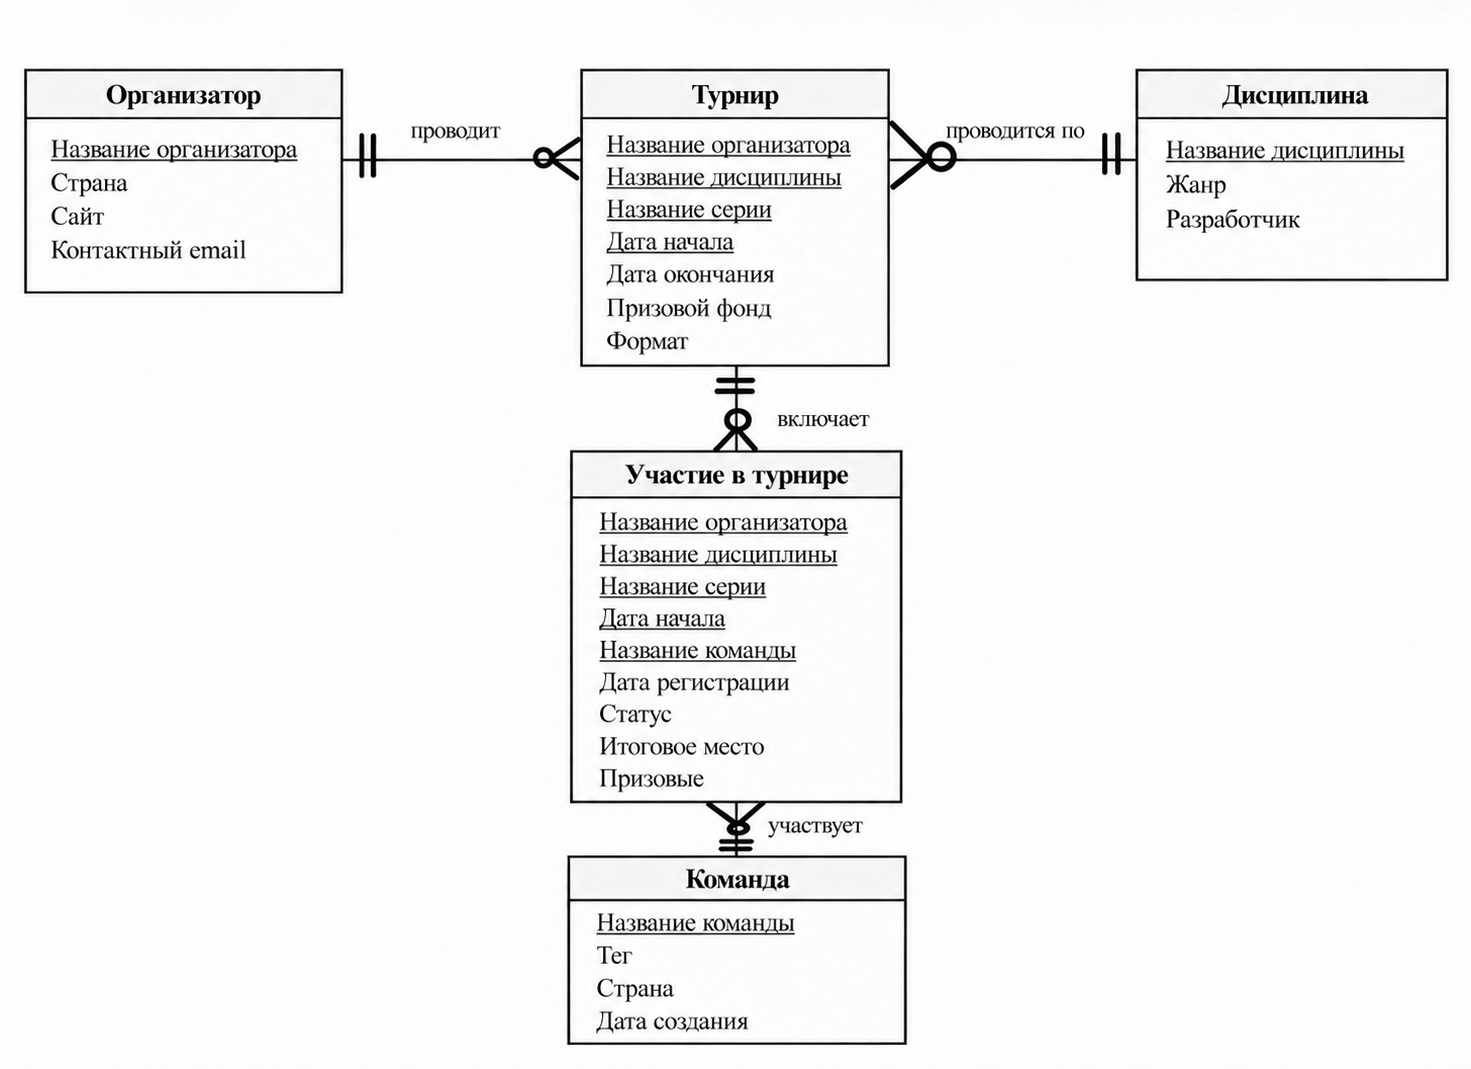
\includegraphics[width=0.9\textwidth]{labdb1.png}
  \caption{Модель «сущность-связь»}
\end{figure}

Между описанными сущностями были построены связи, согласующиеся с особенностями предметной области:

\begin{itemize}
  \item \textbf{Организатор - Турнир:} так как организатор может проводить несколько различных турниров, а каждый турнир проводится строго одним организатором, то выбрана связь «один-ко-многим». Минимальные кардинальные числа равны 0 и 1, так как у организатора могут временно отсутствовать турниры, а каждому турниру должен соответствовать организатор.

  \item \textbf{Дисциплина - Турнир:} так как по одной дисциплине может проводиться несколько различных турниров, а каждый турнир проводится строго по одной дисциплине, то выбрана связь «один-ко-многим». Минимальные кардинальные числа равны 0 и 1, так как по дисциплине могут временно отсутствовать турниры, а каждому турниру должна соответствовать дисциплина.
\end{itemize}



\begin{itemize}
  \item \textbf{Турнир - Участие в турнире:} так как турнир может включать несколько записей об участии команд, а каждая запись об участии относится строго к одному турниру, то выбрана связь «один-ко-многим». Минимальные кардинальные числа равны 0 и 1, так как в турнире могут временно отсутствовать зарегистрированные команды, а каждой записи об участии должен соответствовать турнир.

  \item \textbf{Команда - Участие в турнире:} так как команда может участвовать в нескольких различных турнирах, а каждая запись об участии относится строго к одной команде, то выбрана связь «один-ко-многим». Минимальные кардинальные числа равны 0 и 1, так как команда может ещё не участвовать в турнирах, а каждой записи об участии должна соответствовать команда.
\end{itemize}

\end{document}
